\documentclass[aspectratio=169]{beamer}
\setbeamertemplate{navigation symbols}{}
\mode<beamer>{\setbeamertemplate{blocks}[rounded][shadow=true]}

\mode<presentation> {
\usetheme{Goettingen}
\setbeamertemplate{footline}
}

\usepackage{graphicx}
\usepackage{booktabs}
\usepackage{sidecap}
\usepackage{caption}
\usepackage[utf8]{inputenc}
\usepackage[T2A]{fontenc}
\usepackage{chemformula}
%%%
% XXX: the Russian module for babel defines \ch for the hyperbolic cosine operator.
% This conflicts chemformula \ch. Alas babel defines \ch as a "robust"
% command and my TeX-foo is not enough to undefine it. Instead I "rename"
% chemformula's \ch to \Ch to avoid the problem.
\let\Ch\ch
\let\ch\relax
%%%
\usepackage[russian,english]{babel}
\usepackage[warn]{mathtext}
\usepackage{xcolor}
\usepackage{chngpage}
\usepackage{calc}
\RequirePackage[absolute, overlay]{textpos}
\setlength{\TPHorizModule}{\paperwidth}
\setlength{\TPVertModule}{\paperheight}

\title[Армагеддон был вчера]{Армагеддон был вчера}

\author{}
\date{}

\begin{document}

{
\setbeamertemplate{navigation symbols}{}
\usebackgroundtemplate{%
\vbox to \paperheight{\vfil\hbox to \paperwidth{\hfil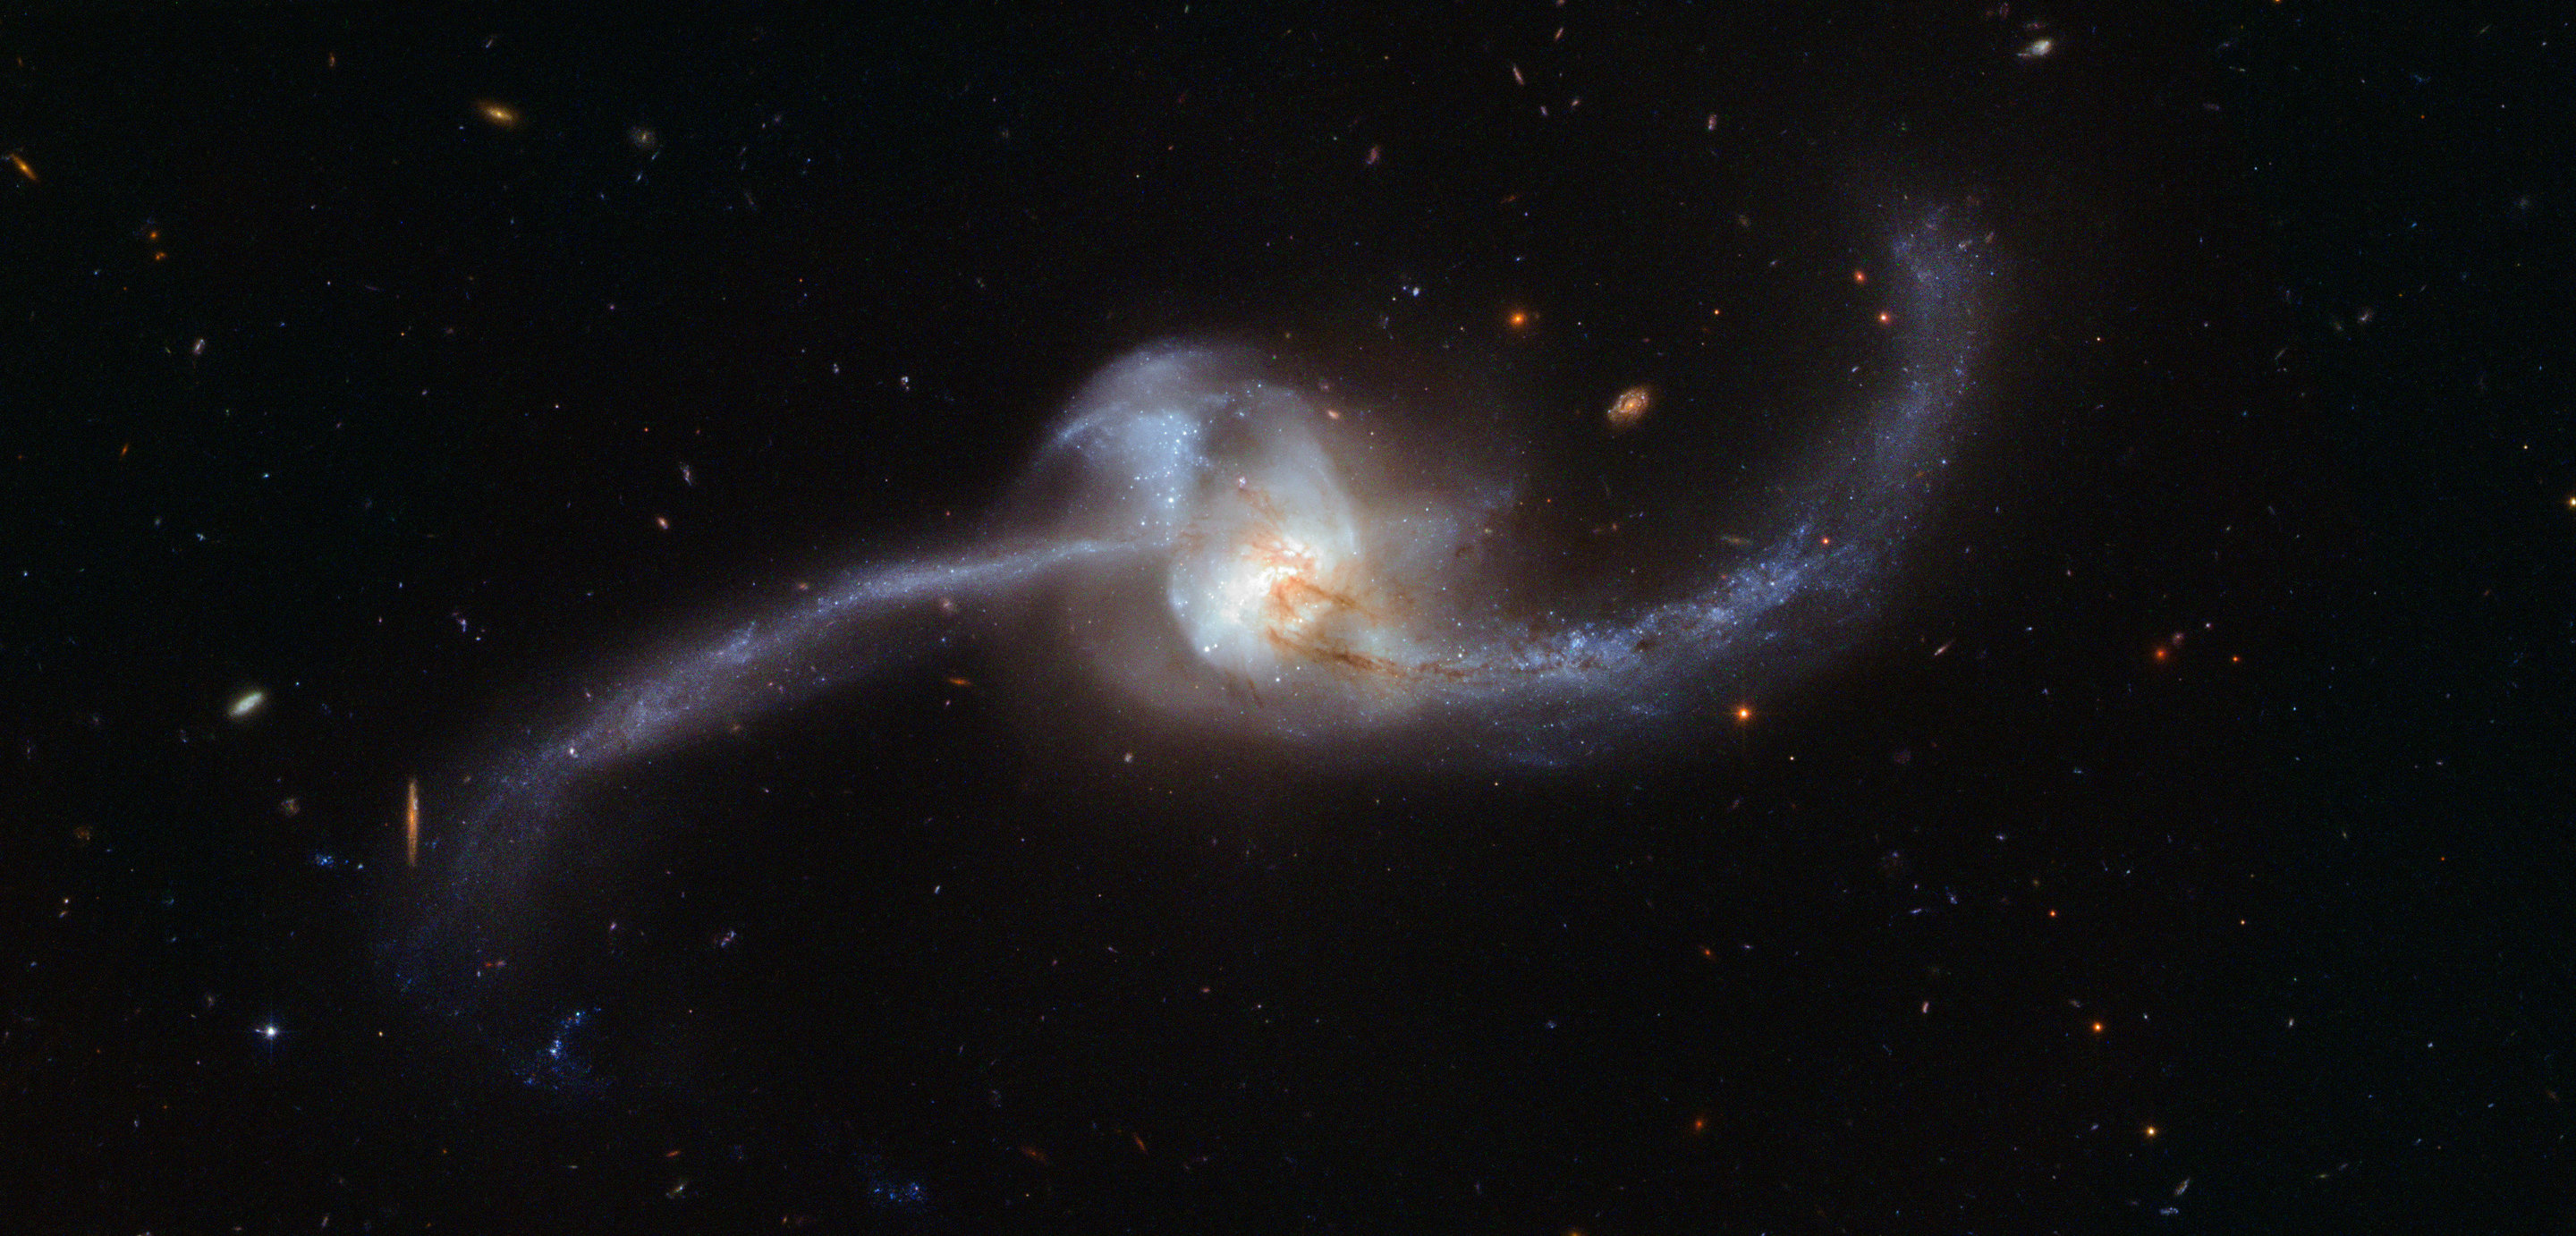
\includegraphics[width=\paperwidth]{img/NGC2623.jpg}\hfil}\vfil}
}
\begin{frame}[plain]
\begin{textblock}{0.4}(0.3,0.1)
\centerline{\scalebox{2.5}{\textcolor{red}{Армагеддон был вчера}}}
\end{textblock}
\begin{textblock}{0.4}(0.3,0.93)
\centerline{\scalebox{1.2}{конец света с точки зрения физики}}
\end{textblock}
\end{frame}
}

{
\usebackgroundtemplate{%
\vbox to \paperheight{%
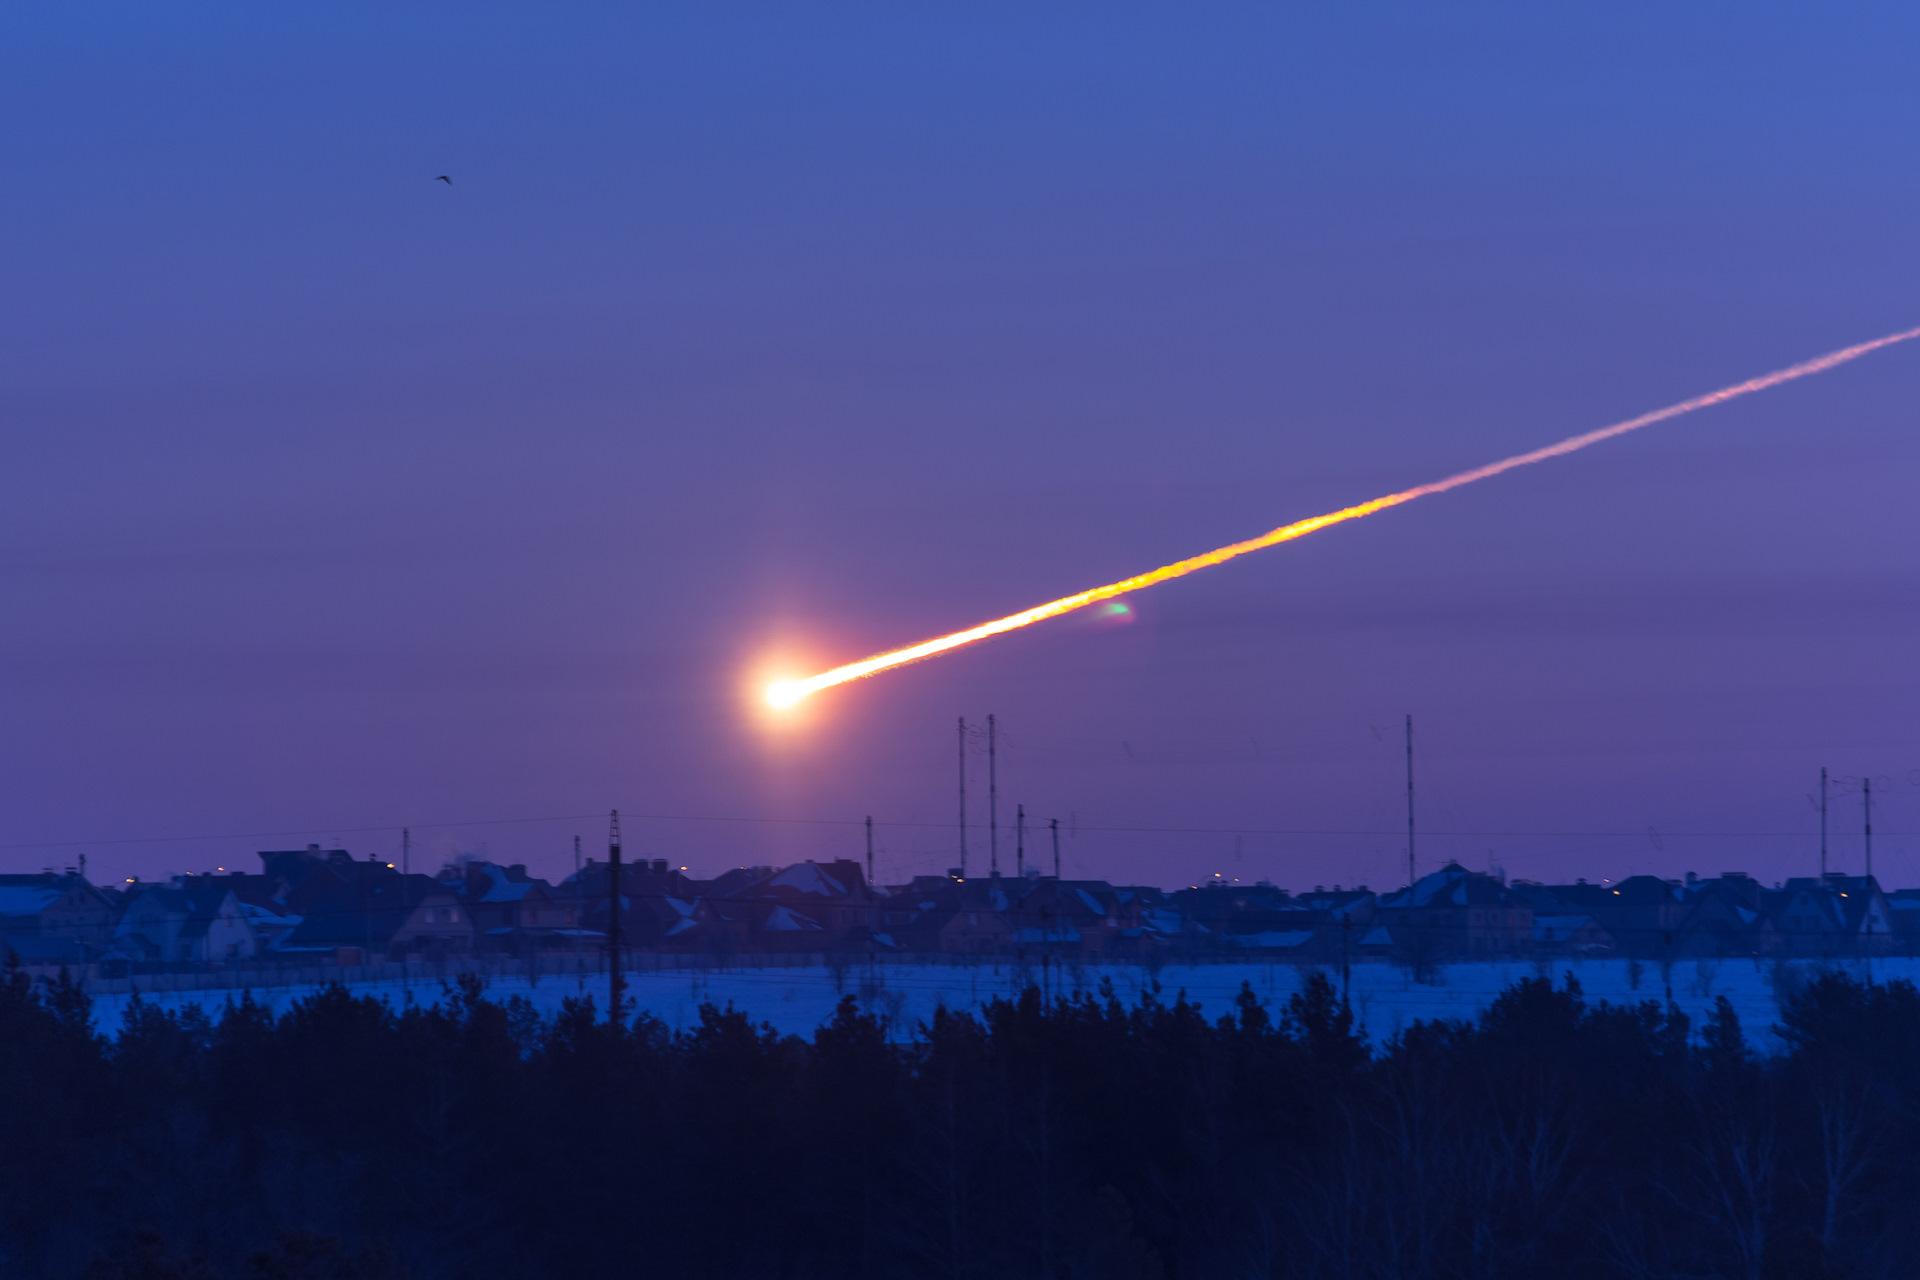
\includegraphics[width=\paperwidth,height=\paperheight,keepaspectratio]{img/chelyabinsk_meteor.jpg}
\vfill
}}
\begin{frame}
\begin{columns}[T]
\column{0.5\textwidth}
{\setbeamercolor{structure}{fg=brown!20}
\vspace{10pt}%
\tableofcontents}
\column{0.5\textwidth}
\vbox to \paperheight{
\vspace{10pt}
\vfill
}
\end{columns}
\end{frame}
}

\section{Определение и классификация}

\begin{frame}
\frametitle{Что такое Конец Света?}
\begin{columns}[c]
\column{0.55\textwidth}
\begin{block}{Массовое вымирание видов}
      \begin{itemize}
        \item Столкновения с астероидами
        \item Взрывы сверхновых
        \item Гамма-всплески
      \end{itemize}
\end{block}
\begin{block}{Полное разрушение биосферы}
      \begin{itemize}
      \item Смещение обитаемой зоны
      \end{itemize}
\end{block}
\begin{block}{Физическое разрушение Земли}
      \begin{itemize}
      \item Солнце -- красный гигант
      \end{itemize}
\end{block}
\column{0.45\textwidth}
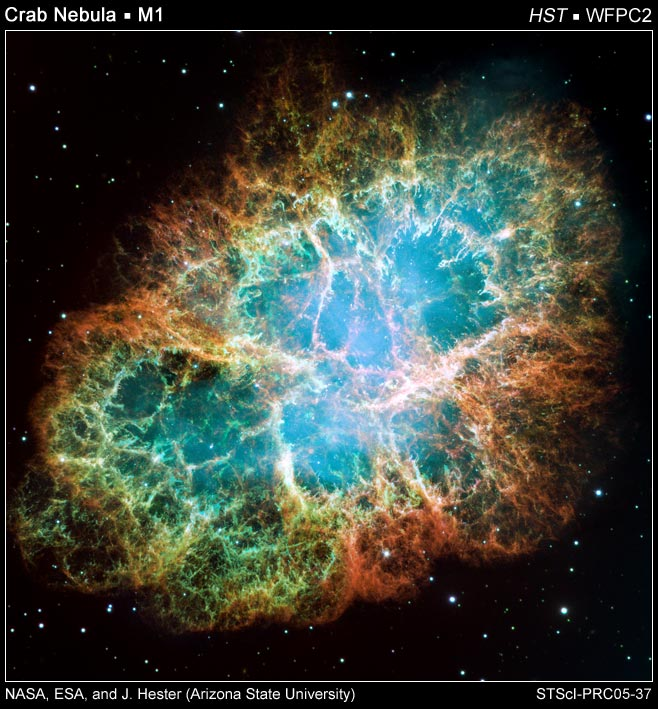
\includegraphics[width=0.95\textwidth]{img/crab_nebula_web_print.jpg}
\end{columns}
\end{frame}

\section{Столкновения с астероидами}

\begin{frame}
\frametitle{Столкновения с астероидами}
\begin{columns}[T]
\column{0.5\textwidth}
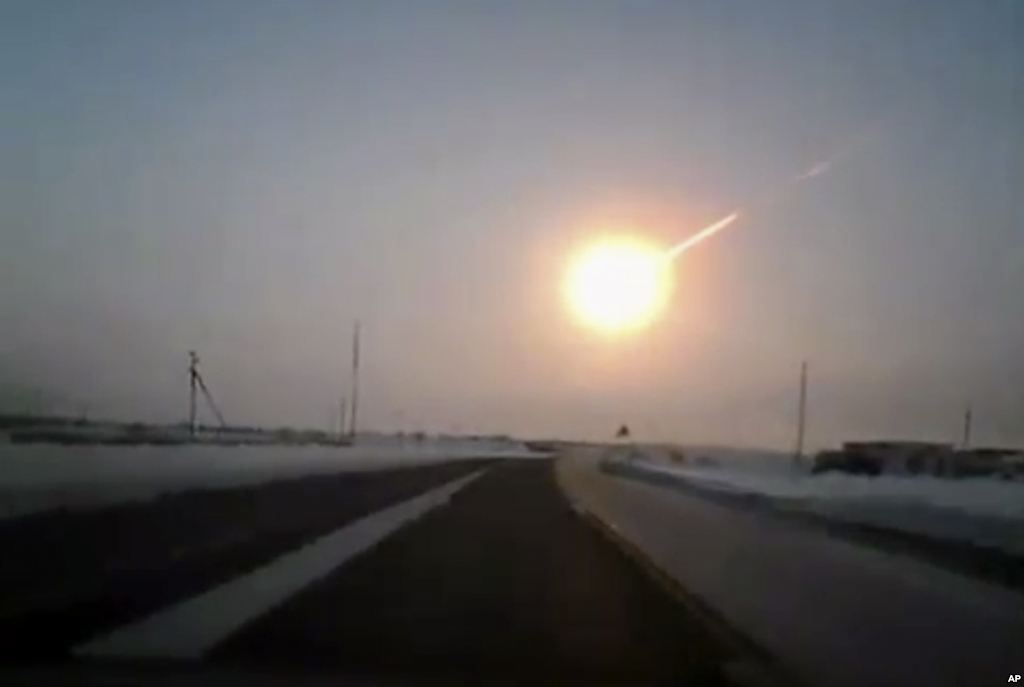
\includegraphics[width=0.95\textwidth]{img/chelyabinsk_meteor_2.jpg}
\column{0.5\textwidth}
\begin{block}{Хорошо, что пополам}
$E = \frac{m v^2}{2} = \frac{2}{3} \pi \rho R^3 v^2$ \\
$\rho \sim 3000 \: \mathrm{\text{кг}/\text{м}^3}$ {\small (гранит)} \\
$v \sim 30 - 80 \: \mathrm{\text{км}/\text{сек}}$ {\small (Солнечная система)} \\
{\Large \color{red} $E \sim 10 \: \mathrm{\text{МТ}}$} \\
$1 \: \mathrm{\text{МТ}} = 4.18 \cdot 10^{15} \mathrm{\text{Дж}}$
\end{block}
\end{columns}
\begin{columns}[c]
\column{0.5\textwidth}
\begin{block}{Один раз в 100 лет}
\begin{itemize}
\item 2013 Челябинский метеорит
\item 1908 Тунгусский метеорит (?)
\end{itemize}
\end{block}
\column{0.5\textwidth}
\begin{block}{Размер имеет значение}
$D < 10 \, \mathrm{\text{м}}$: испаряются в атмосфере
$D \geq 20 - 100 \, \mathrm{\text{м}}$: наземный бабах
\end{block}
\end{columns}
%}
\end{frame}


\begin{frame}
\frametitle{Никто не уйдёт обиженный}

\begin{block}{Диаметр $\sim 500 \: \mathrm{\text{м}}$ (раз в $\sim 50000$ лет)}
\begin{itemize}
\item Энерговыделение: разом взорвать весь (термо)ядерный арсенал.
\item Хватит на целый континент.
\end{itemize}
\end{block}

\begin{block}{Диаметр 2 -- 3 км (раз в несколько миллионов лет)}
\begin{itemize}
\item Выбрасывает и распыляет огромные массы земной коры.
\item Пыль остаётся в атмосфере годы -- глобальное похолодание.
\end{itemize}
\end{block}

\begin{block}{Диаметр 5 -- 10 км (раз в $\sim 100$ миллионов лет)}
\begin{itemize}
\item Ядерная зима на десятилетия, закисление океанов
\item Мело-палеогеновое вымирание (бедные динозаврики)
\end{itemize}
\end{block}
\end{frame}

{
\usebackgroundtemplate{
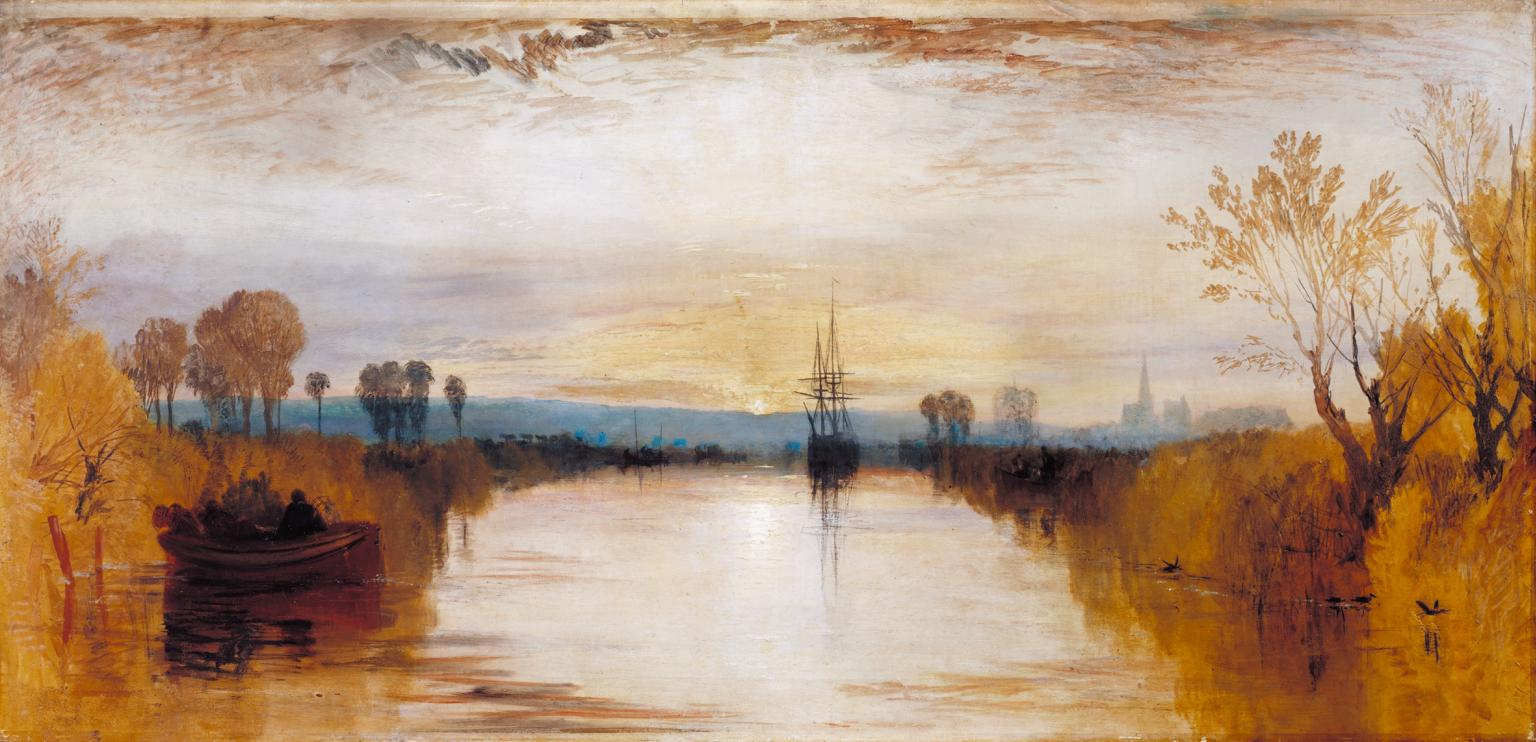
\includegraphics[width=\paperwidth,height=0.75\paperheight,keepaspectratio]{img/Chichester_Canal_1828.jpg}
}
\begin{frame}
\frametitle{Год без лета, 1816}
%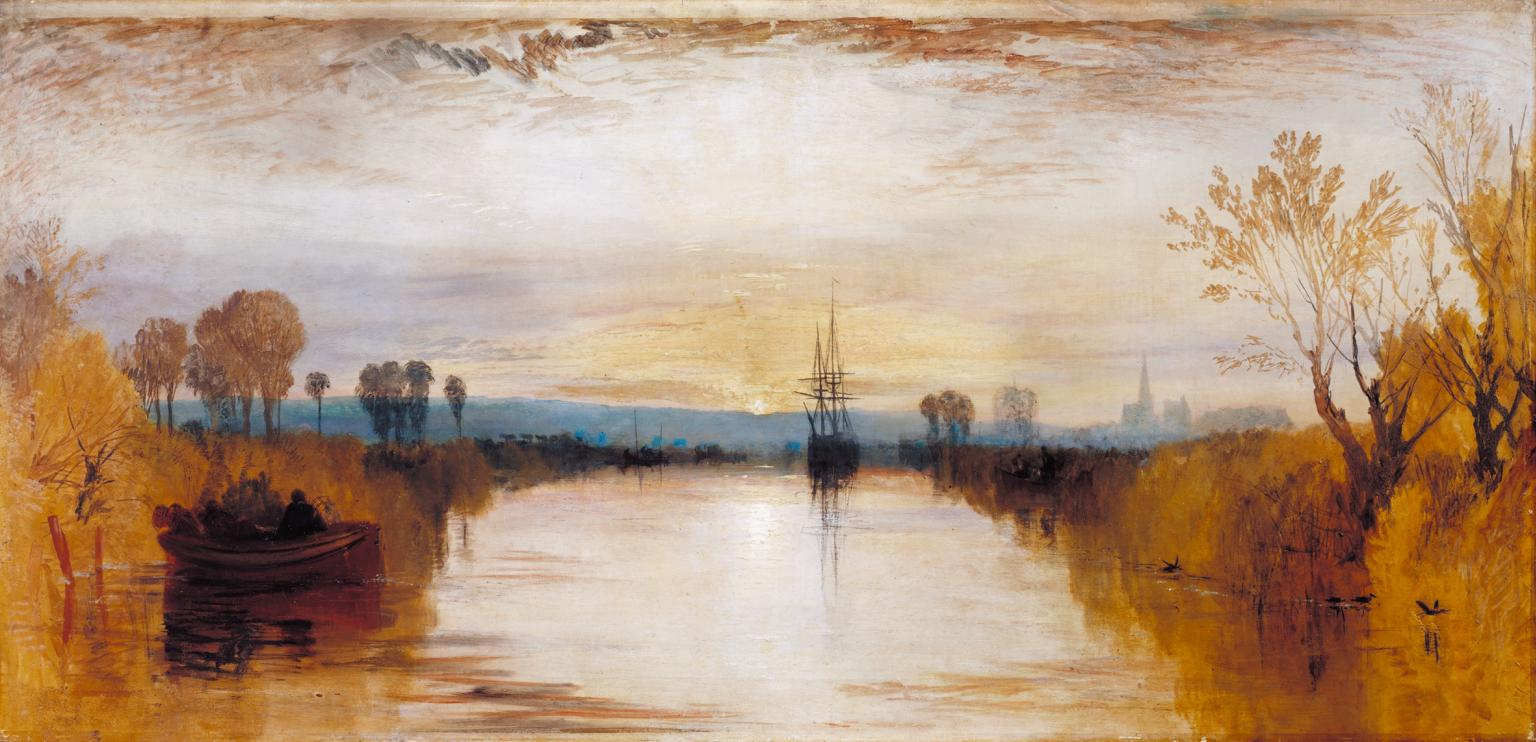
\includegraphics[width=\textwidth]{img/Chichester_Canal_1828.jpg}
\only<1>{
\begin{textblock}{1}(0.0,0.75)
\begin{center}
\tiny{``Чичестерский канал'', Уильям Тёрнер, 1828}
\end{center}
\end{textblock}
}
\only<2>{
\begin{textblock}{0.5}(0.02,0.73)
\begin{block}{Апрель 1815г}
Извержение вулкана Тамбора (Индонезия)
\end{block}
\end{textblock}
}
\only<3>{
\begin{textblock}{0.35}(0.02,0.73)
\begin{block}{Март 1816г}
В Европе зима
\end{block}
\end{textblock}
}
\only<4>{
\begin{textblock}{0.4}(0.02,0.73)
\begin{block}{Апрель, май 1816г}
сплошные дожди и град в Европе
\end{block}
\end{textblock}
}
\only<5>{
\begin{textblock}{0.35}(0.02,0.73)
\begin{block}{Июнь, июль 1816г}
В Нью-Йорке выпадал снег
\end{block}
\end{textblock}
}
\end{frame}
}

\section{Взрывы сверхновых}

\begin{frame}
\frametitle{Взрывы сверхновых}
\only<1>{
\begin{columns}[c]
\column{0.55\textwidth}
\begin{figure}
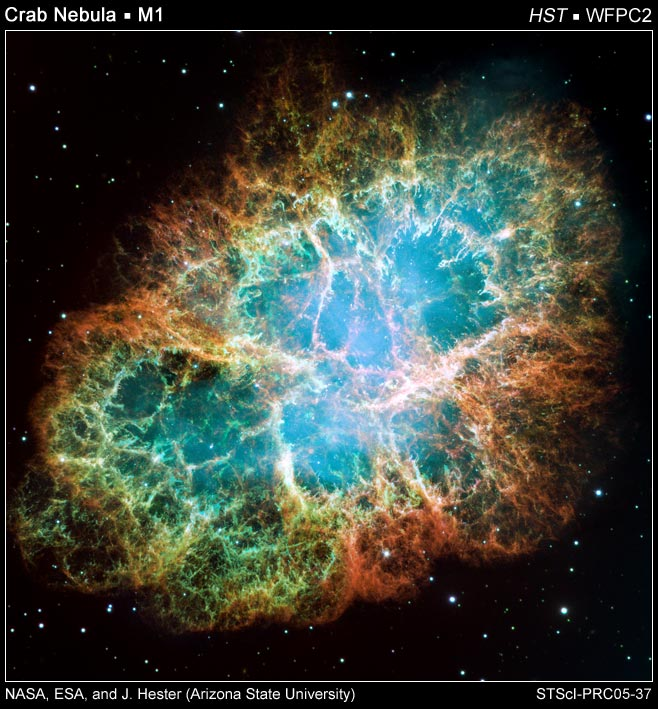
\includegraphics[width=0.95\textwidth]{img/crab_nebula_web_print.jpg}
\end{figure}
\column{0.45\textwidth}
\begin{block}{Крабовидная туманность}
\begin{itemize}
\item Наблюдали $\approx$ 1054 год
\item Была видна даже днём
\item размер: $\approx 11 \, \mathrm{\text{св.~лет}}$
\item расстояние: $\approx 6500 \, \mathrm{\text{св.~лет}}$ 
\end{itemize}
\end{block}
\end{columns}
}
\only<2>{
\begin{itemize}
\item Тяжелые звёзды ($M > 8 M_\odot$) коллапсируют в конце жизни
\item Сжатие вызывает огромный термоядерный взрыв
\item Сверхновая ярче целой галактики (на несколько недель)
\item Мощный источник ЭМ излучения и частиц сверхвысоких энергий
\item Угроза всему живому на расстоянии менее 10 -- 50 св. лет
\end{itemize}
\begin{block}{Со мной такое точно не случится}
\begin{itemize}
\item В Млечном Пути сверхновые взрываются раз в 50 лет
\item Рядом с нами {\bf пока} нет таких массивных звёзд так близко
\item В будущем Солнце может переместиться в менее спокойное место
\end{itemize}
\end{block}
}
\end{frame}

\begin{frame}
\frametitle{Чем именно опасны сверхновые}
\begin{block}{Глобальное похолодание}
\begin{itemize}
\item $\gamma$-лучи разбивают на атомы молекулы воздуха $\Ch{N2}$ и $\Ch{O2}$
\item Из атомарного азота и кислорода образуются оксиды азота $\Ch{NO}$, $\Ch{NO2}$
\item Эти молекулы могут находится в стратосфере годами
\item $\Ch{NO2}$ хорошо поглощает видимый свет
\end{itemize}
\end{block}

\begin{block}{Повышение уровня солнечного УФ излучения}
\begin{itemize}
\item $\Ch{NO}$ разрушает озон: $\Ch{NO} + \Ch{O3} \to \Ch{NO2} + \Ch{O2}$
\item Уровень солнечного УФ на поверхности Земли повышается
\item Увеличение уровня УФ на 30\%: смерть фитопланктона (прощай, кислород)
\end{itemize}
\href{https://руни.рф/index.php/\%D0\%9E\%D1\%80\%D0\%B4\%D0\%BE\%D0\%B2\%D0\%B8\%D0\%BA\%D1\%81\%D0\%BA\%D0\%BE-\%D1\%81\%D0\%B8\%D0\%BB\%D1\%83\%D1\%80\%D0\%B8\%D0\%B9\%D1\%81\%D0\%BA\%D0\%BE\%D0\%B5_\%D0\%B2\%D1\%8B\%D0\%BC\%D0\%B8\%D1\%80\%D0\%B0\%D0\%BD\%D0\%B8\%D0\%B5}{Ордовикско-силурийское вымирание} (440 миллионов лет назад) \cite{arXiv:astro-ph/0309415}
\end{block}
\end{frame}


\section{Гамма-всплески}
\begin{frame}
\frametitle{Гамма-всплески}
\begin{block}{Взрывы быстро вращающихся звёзд}
\begin{itemize}
\item Во время взрыва создаются мощные магнитные поля
\item Магнитные поля фокусируют продукты взрыва
\item Узкие потоки могут быть опасны даже на $\sim 10000$~СЛ
\end{itemize}
\end{block}
\begin{block}{А также}
\begin{itemize}
\item Слияния нейтронных звёзд
\item Слияния чёрных дыр
\end{itemize}
\end{block}
\end{frame}


\begin{frame}
\frametitle{Техника безопасности при работе с гамма-вслесками}
\begin{block}{Не пытайтесь повторить дома!}
 GRB~221009A: $E_{iso} \sim 6.5 \times M_\odot \approx 1.2 \times 10^{47} \mathrm{\text{Дж}} \approx 3.5 \times 10^{32} \mathrm{\text{МТ}}$  \cite{arXiv:2302.13383}
\end{block}

\begin{block}{Нужно ли прятаться в радиационное убежище?}
\begin{enumerate}
\item Поздно метаться: всплеск длится секунды -- минуты ($v = c$)
\item Атмосфера задерживает излучение, опасны отдалённые последствия
\end{enumerate}
\end{block}

\begin{block}{Есть ли что-то опасное рядом?}
Звезда Вольфа -- Райе \href{https://en.wikipedia.org/wiki/WR_104}{WR 104}, 8000 св.~лет
\end{block}

\begin{block}{Как часто случаются близкие к Земле гамма-вспышки?}
Примерно раз в миллиард лет (очень грубая оценка)
\end{block}
\end{frame}


\section{Смещение обитаемой зоны}
\begin{frame}
\frametitle{Гори, гори, моя звезда}
\only<1>{
\begin{columns}[c]
\column{0.4\textwidth}
\begin{block}{Ядро}
Ядерные реакции: $4p \to \alpha$ \\
$\varnothing \approx 20 \% \; \varnothing_\odot$ \\
$\mathrm{M} \approx 30 - 40 \% \; \mathrm{M}_\odot$ \\
\end{block}
\begin{block}{Зона лучистого переноса}
Энергию переносит свет \\
За миллионы лет
\end{block}
\begin{block}{Конвективная зона}
Перенос энергии потоками вещества
\end{block}
\vfill
\column{0.6\textwidth}
\begin{figure}
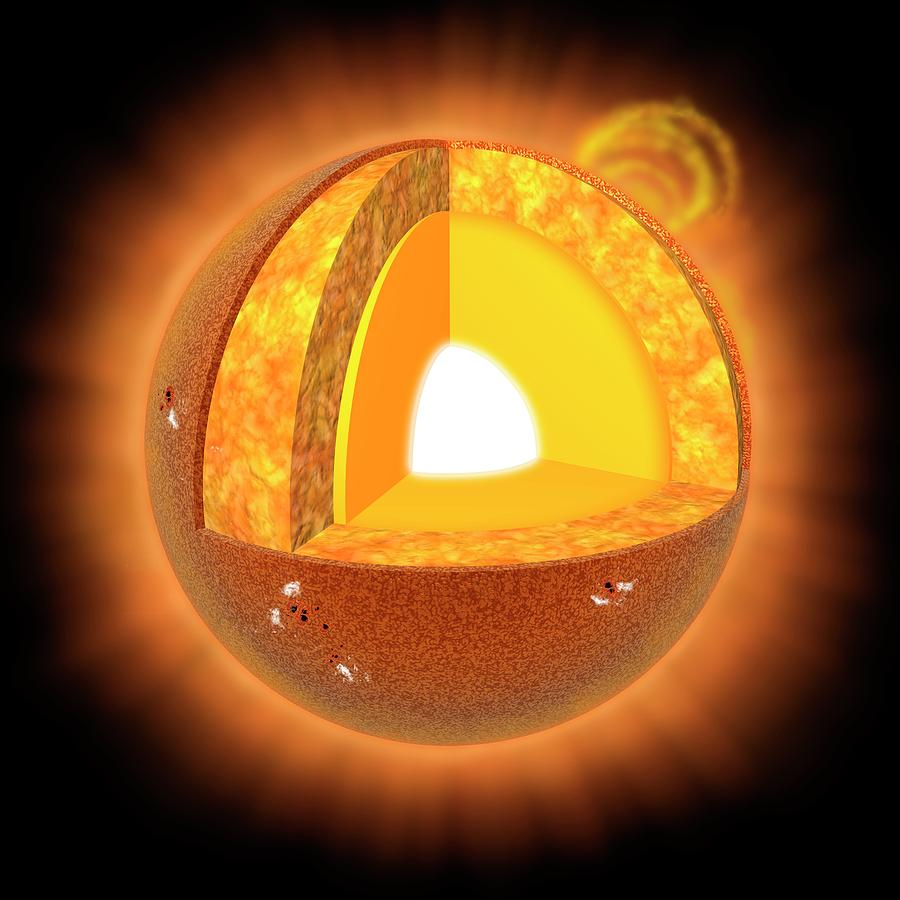
\includegraphics{img/sun_structure.jpg} \\
\captionsetup{labelformat=empty}
\caption{Звезда главной последовательности}
\end{figure}
\end{columns}
}
\only<2>{
\begin{columns}[c]
\column{0.45\textwidth}
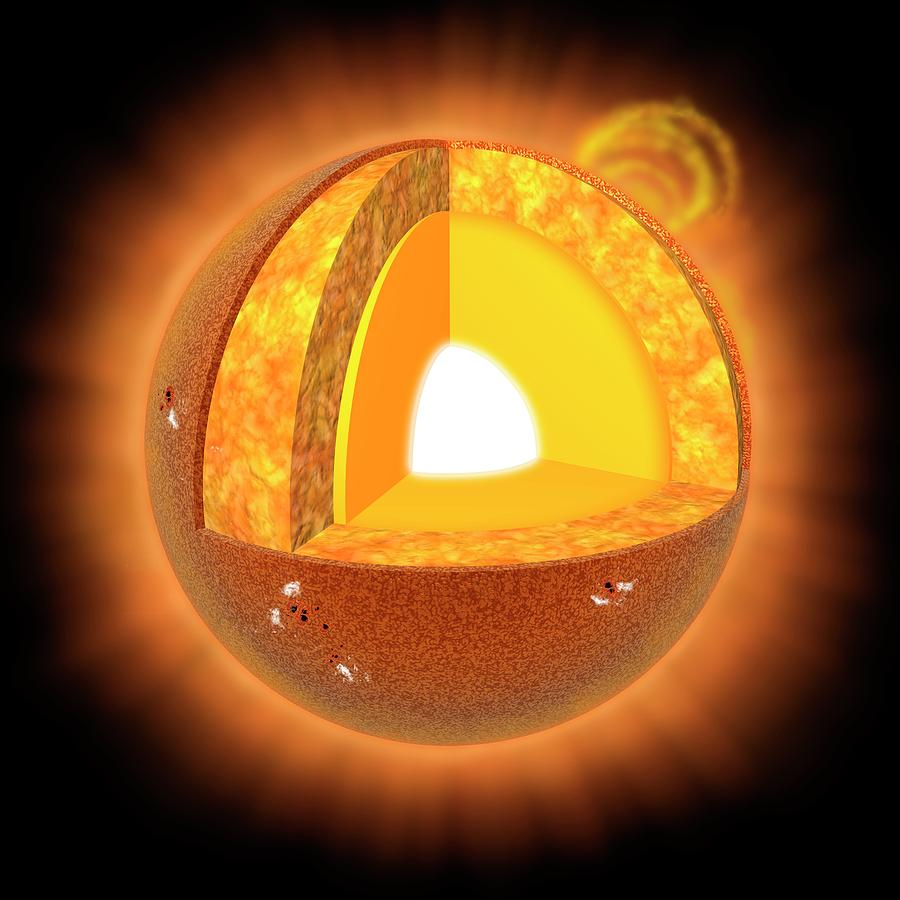
\includegraphics[width=\textwidth]{img/sun_structure.jpg}
\column{0.55\textwidth}
\begin{block}{Устойчивое равновесие}
\begin{itemize}
\item Водород выгорает
\item Синтез временно замедляется
\item Сжатие (гравитация)
\item Рост давления и температуры
\item Синтез ускоряется
\item Снова равновесие
\end{itemize}
\end{block}
\begin{block}{Со временем ...}
\begin{itemize}
\item Ядро сжимается и нагревается
\item Внешние слои слегка расширяются
\item На 1\% ярче каждые 100 млн. лет
\end{itemize}
\end{block}
\end{columns}
}
\end{frame}

\begin{frame}
\frametitle{Эволюция Солнца на главной последовательности}
\begin{figure}
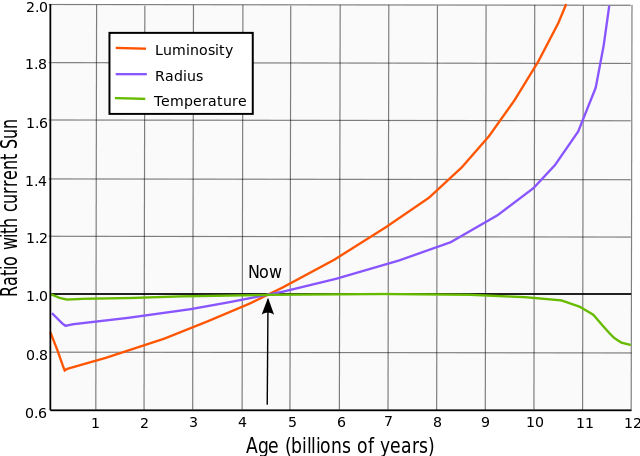
\includegraphics[width=0.7\textwidth]{img/640px-Solar_evolution_(English).png}
\captionsetup{labelformat=empty}
\caption{Изменение светимости, радиуса, и температуры Солнца\cite{arXiv:0911.4872}}
\end{figure}
\end{frame}


\begin{frame}{Прекращение фотосинтеза}
\begin{block}{Базальт}
\begin{itemize}
\item Большинство вулканических пород, океаническая кора
\item 47 -- 52\% $\Ch{SiO2}$, 14 --18\% $\Ch{Al2O3}$, {\bf 6 --12\% $\Ch{CaO}$}
\end{itemize}
\end{block}
Атмосферный $\Ch{CO2}$ медленно превращается в известняки:
\begin{displaymath}
\nonumber
\Ch{CaSiO3} + \Ch{CO2} + \Ch{H2O} \to 2 \Ch{HCO3-} + \Ch{Ca^{2+}} + \Ch{SiO2}
\end{displaymath}

\begin{itemize}
\item Скорость реакции быстро растёт с температурой
\item Концентрация $\Ch{CO2}$ через 600 млн. лет: 50 ЧНМ (сейчас: 400 ЧНМ)
\item 50 ЧНМ не достаточно для $C_3$ фиксации
\item Подавляющее большинство растений живут за счёт $C_3$ процесса
\item Растения использующие $C_4$ фиксацию вымрут ещё через 200~млн.~лет
\end{itemize}

\end{frame}

\begin{frame}
\frametitle{Потеря океанов}
В наше время: $T_{\bigoplus} \approx 287 \mathrm{K} = 14^\circ \mathrm{C}$
\begin{block}{Увеличение светимости Солнца на 10\%}
\begin{itemize}
\item Температура поверхности Земли поднимается до $320 \mathrm{K}$ ($47^\circ \mathrm{C}$)
\item Увеличивается содержание водяного пара в атмосфере
\item Всё больше водяного пара достигает стратосферы
\item Солнечный УФ разбивает воду на кислород и водород
\item Лёгкие молекулы водорода улетают в космос
\item Результат: потеря океанов через миллиард лет \cite{James F. Kasting}
\end{itemize}
Океаны при этом не кипят.
\end{block}
\end{frame}


\section{Слияние Млечного Пути и Андромеды}
{
\setbeamertemplate{navigation symbols}{}
\usebackgroundtemplate{%
\vbox to \paperheight{%
\vspace*{30pt}
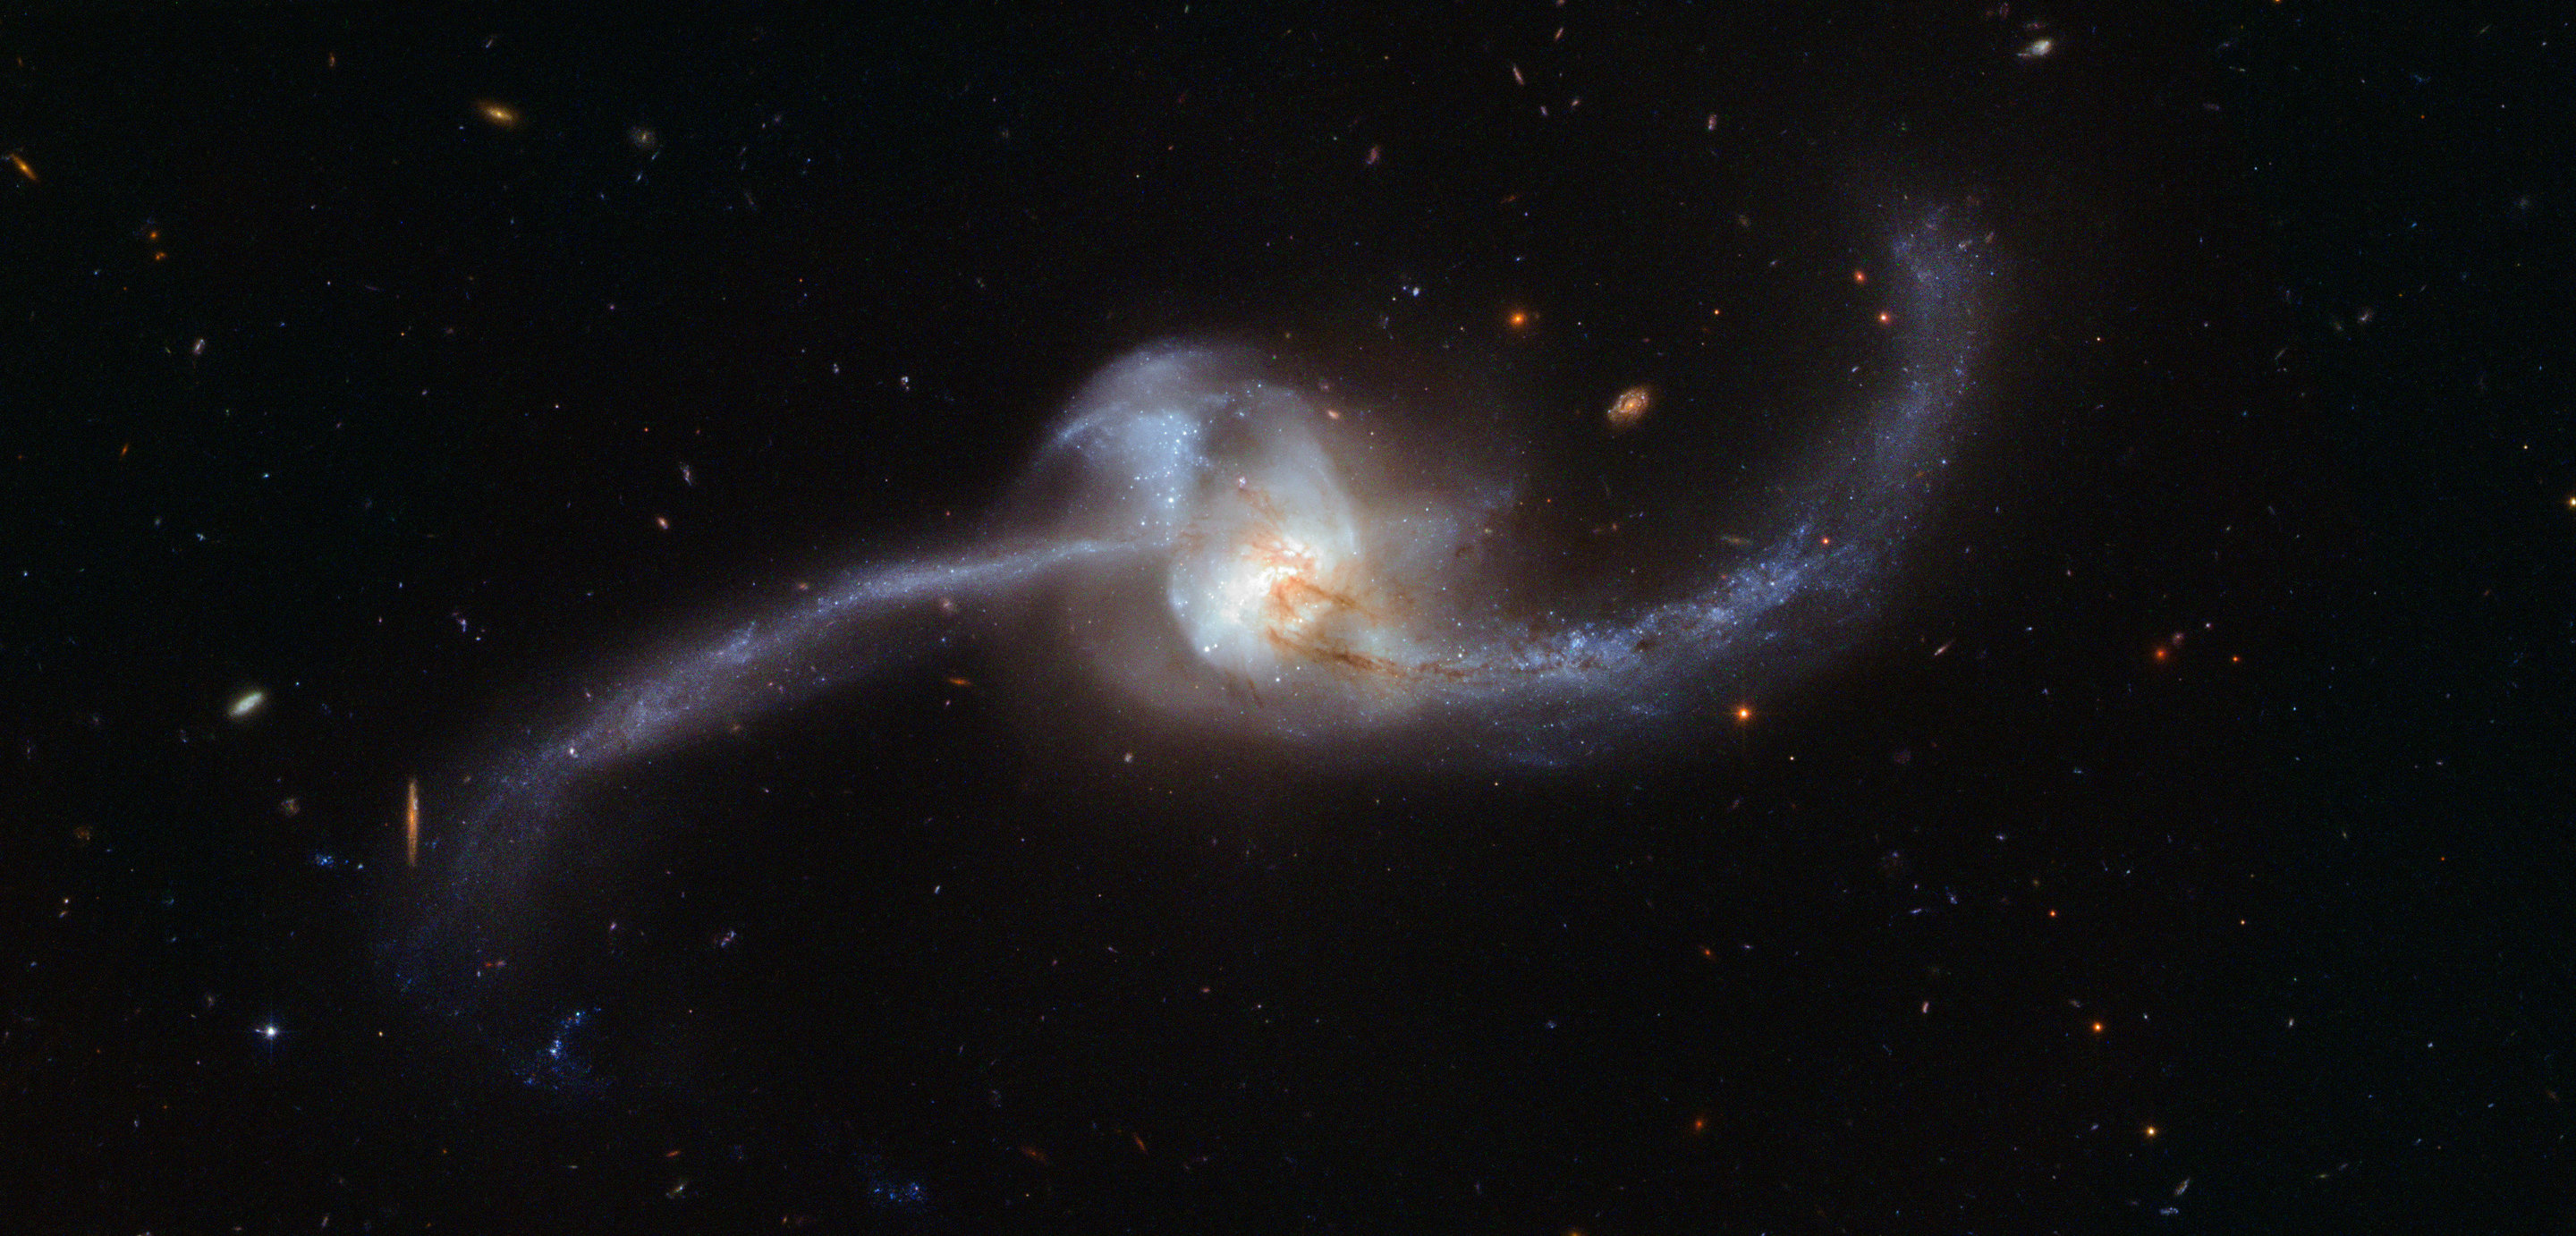
\includegraphics[width=\paperwidth,height=\paperheight,keepaspectratio]{img/NGC2623.jpg}
\vfill
}}
\begin{frame}[fragile]
\frametitle{Слияние галактик, NGC 2623}
\begin{textblock}{0.5}(0.05,0.35)
\begin{centering}
\textcolor{red}{255 млн. св. лет}
\end{centering}
\end{textblock}
\end{frame}
}

\begin{frame}
\frametitle{Слияние галактик, Млечный Путь и Андромеда}
\only<1>{
\begin{figure}
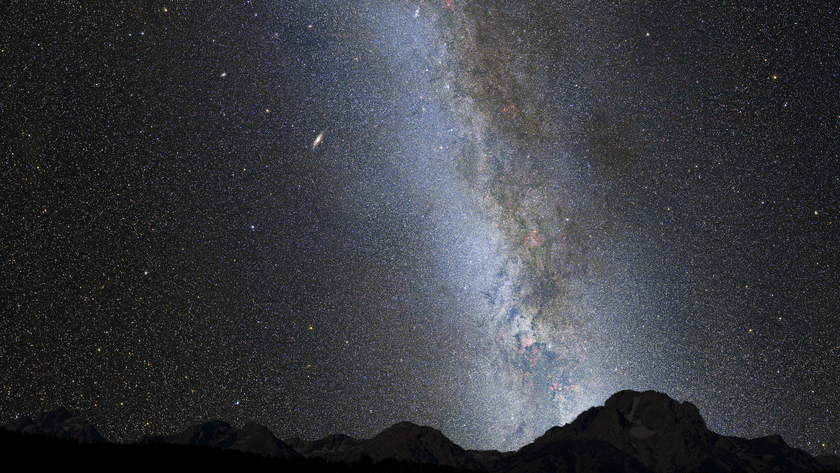
\includegraphics[width=\textwidth]{img/20120929_andromeda_collision_1-present_hs-2012-20-c_f840.png}
\captionsetup{labelformat=empty}
\caption{сейчас}
\end{figure}
}
\only<2>{
\begin{figure}
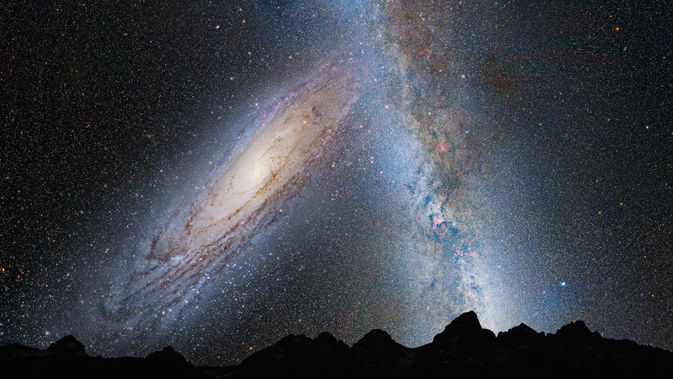
\includegraphics[width=\textwidth]{img/milkdromeda.jpg}
\captionsetup{labelformat=empty}
\caption{через $\sim 3.5$ миллиардов лет}
\end{figure}
}
\transdissolve<2>
\end{frame}

\begin{frame}
\frametitle{Слияние Млечного Пути и Андромеды}
\begin{itemize}
\item Андромеда приближается к нам со скоростью $\sim 110 \: \text{км}/\text{сек}$.
\item Хаббл \cite{arXiv:1205.6864}, Gaia \cite{arXiv:1805.04079}: Андромеда движется на нас ``в лоб''.
\item ожидаемое время: 3,75 -- 4,5 миллиардов лет
\end{itemize}
\begin{columns}[c]
\column{0.4\textwidth}
\begin{block}{Звёзды не сталкиваются}
$D(\alpha \text{Центавра}- \odot) \sim 3 \cdot 10^7 D_\odot$
\end{block}
\column{0.45\textwidth}
\begin{block}{}
\begin{itemize}
\item Изменение орбит звёзд
\item Всплеск звездообразования
\item Перезапуск квазаров
\end{itemize}
\end{block}
\end{columns}
\end{frame}

{
\setbeamercolor{frametitle}{fg=brown!80}
\usebackgroundtemplate{%
\vbox to \paperheight{%
\vspace{4pt}%
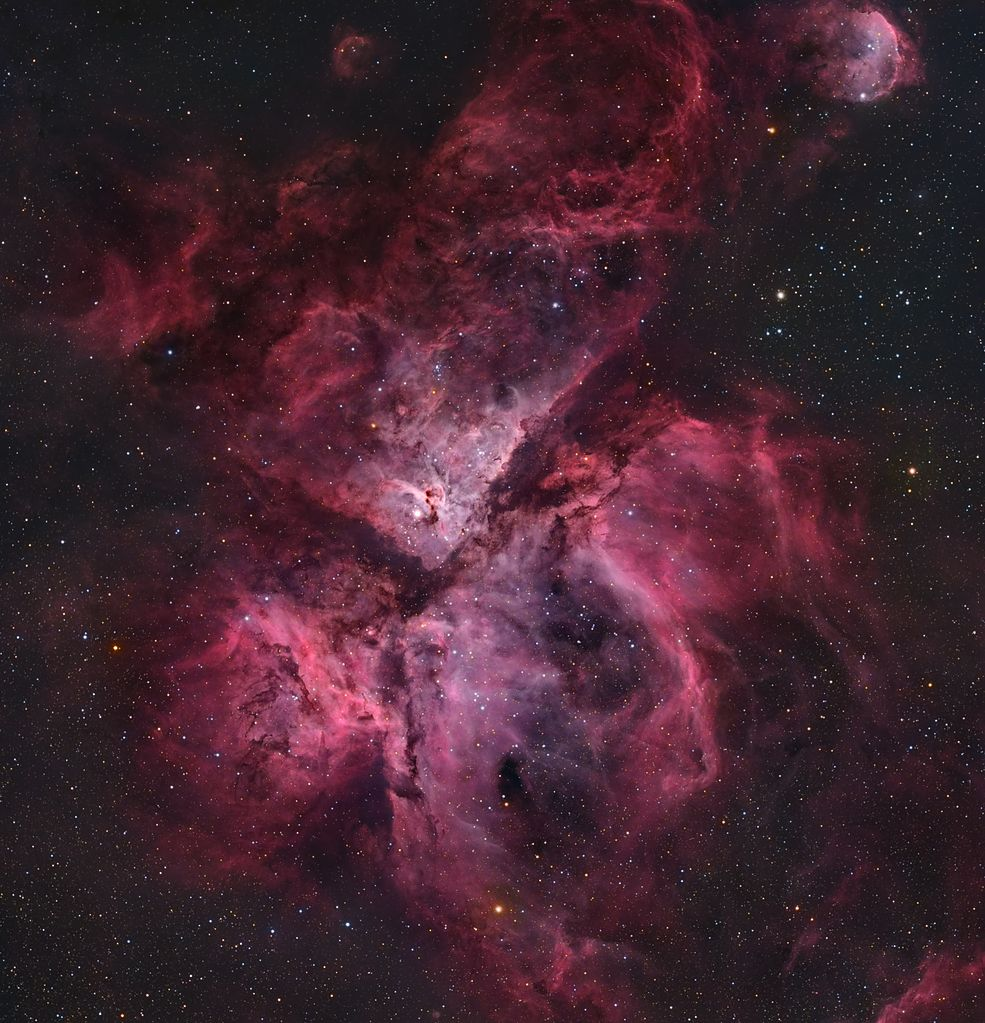
\includegraphics[width=\paperwidth,keepaspectratio,height=\paperheight,angle=90,origin=lB]{img/Carina_Nebula.jpg}\vfill}}
\begin{frame}
\frametitle{Всплеск звездообразования}
\begin{columns}[T]
\column{0.66\textwidth}
\vfill
\column{0.34\textwidth}
\only<1>{
\begin{block}{NGC 3372}
Туманность Киля \\
Eta Carinae nebula
\begin{itemize}
\item $\varnothing = 460 \; \mathrm{\text{св. лет}}$
\item $D = 9000 \; \mathrm{\text{св. лет}}$
\end{itemize}
\end{block}
\begin{block}{Равновесие}
\begin{itemize}
\item Сжате газа
\item Звёздный ветер
\end{itemize}
\end{block}
}
\only<2>{
\begin{block}{Столкновения}
\begin{itemize}
\item $\varnothing \sim 100 \; \mathrm{\text{св. лет}}$
\item Ударные волны
\item Много новых массивных звёзд
\item Сверхновые через $\approx 30\; \mathrm{\text{млн. лет}}$
\end{itemize}
\end{block}
}
\end{columns}
\end{frame}
}

{
\usebackgroundtemplate{
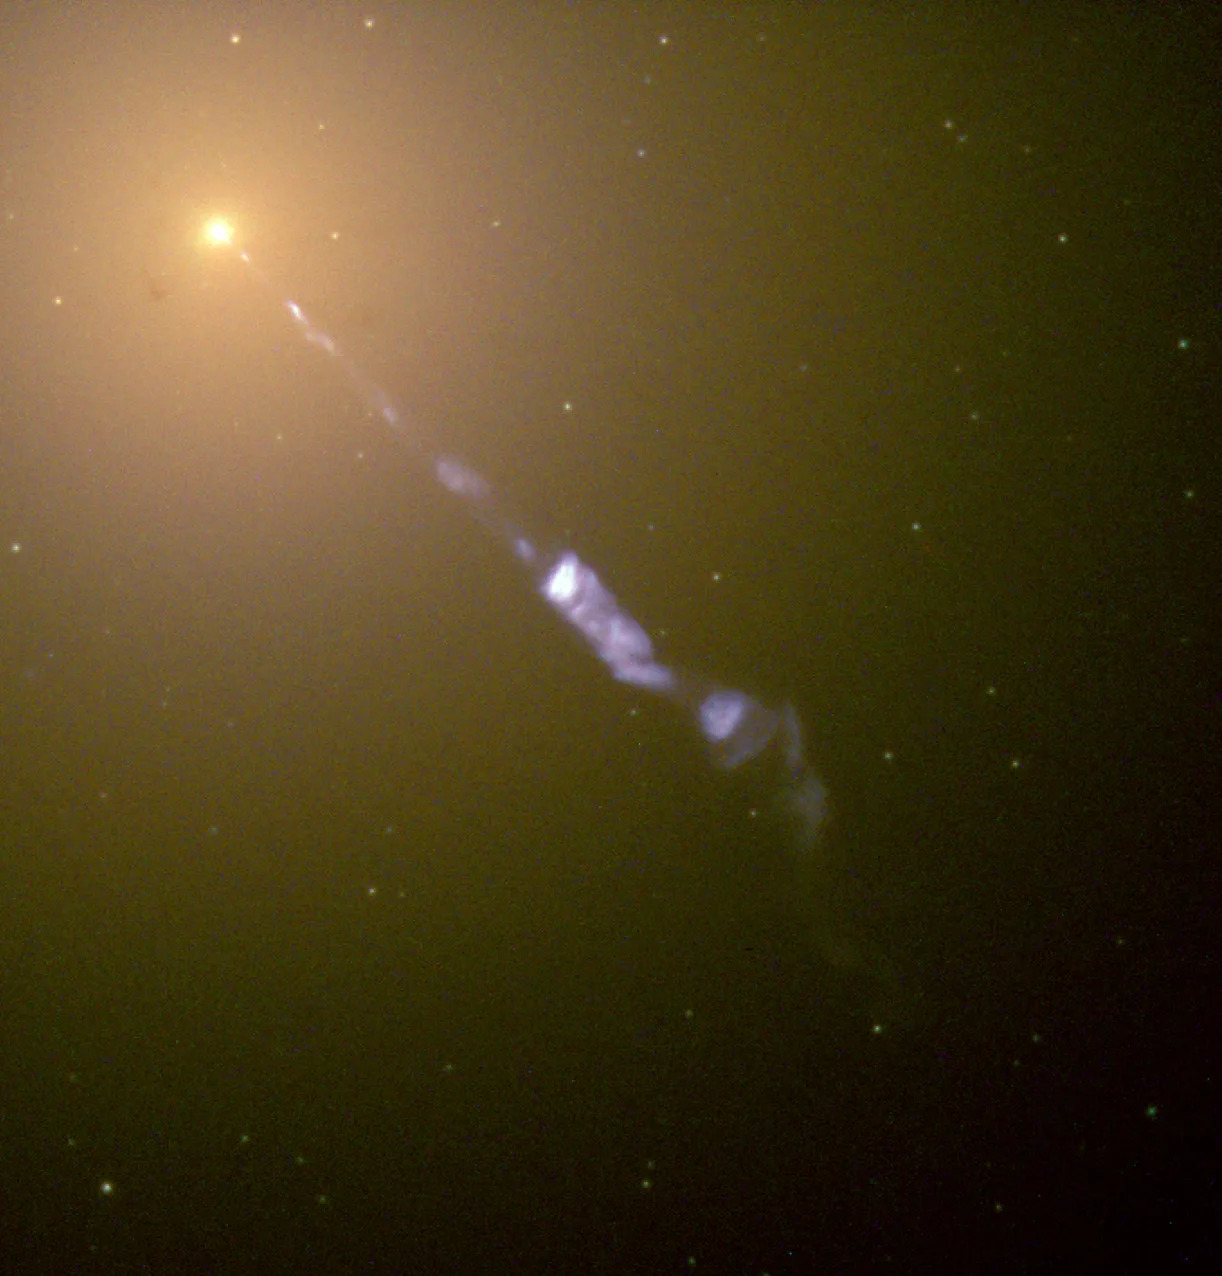
\includegraphics[width=\paperwidth,keepaspectratio]{img/m87jet-jpg.jpg}
}
\begin{frame}
\frametitle{Слияния сверхмассивных чёрных дыр}
\begin{textblock}{0.4}(0.45,0.10)
\begin{block}{}
$\mbox{Sgt }{\mbox{A}^*}: \mathrm{M} \sim 3,6 \cdot 10^6 \mathrm{M}_\odot$ \\
M31: $\mathrm{M} \sim 1 - 2 \cdot 10^8 \mathrm{M}_\odot$ \cite{arXiv:astro-ph/0509839}
\end{block}
\end{textblock}
\begin{textblock}{0.35}(0.50,0.3)
\begin{block}{Обычные звёзды}
\begin{itemize}
\item Разрыв приливными силами
\item Выбрасывание из галактики 
\end{itemize}
Надо попасть: $r_s \approx 10$ АЕ
\end{block}
\begin{block}{Газовые туманности}
Квазар ($\sim 10^7$ сверхновых)
\end{block}
\end{textblock}
\begin{textblock}{0.32}(0.02,0.70)
\begin{block}{$\mbox{M87}^{*}$}
$d = 53,5 \; \mbox{\text{млн. св. лет}}$ \\
$\mathrm{M} \approx 7,2 \cdot 10^9 \, \mathrm{M}_\odot$, $r_s = 120 \; \mbox{\text{АЕ}}$ \\
$L_{jet} \approx 5000 \; \mbox{\text{св. лет}}$
\end{block}
\end{textblock}
\end{frame}
}

\section{Красное Солнышко}
\begin{frame}
\begin{columns}[c]
\column{0.4\textwidth}
\only<1>{
\begin{block}{Ядро}
Ядерные реакции: $4p \to \alpha$ \\
$\varnothing \approx 20 \% \; \varnothing_\odot$ \\
$\mathrm{M} \approx 30 - 40 \% \; \mathrm{M}_\odot$ \\
Гидростатическое равновесие
\end{block}
\begin{block}{Зона лучистого переноса}
Энергию переносит свет \\
За миллионы лет
\end{block}
\begin{block}{Конвективная зона}
Перенос энергии потоками вещества
\end{block}
}
\only<2>{
\begin{block}{В ядре кончился водород}
\begin{itemize}
\item Гелий ещё не ``горит''
\item Синтез в тонком слое вокруг ядра
\item Масса ядра растёт
\end{itemize}
\end{block}
}
\only<3>{
\begin{textblock}{0.3}(0.05,0.0)
\begin{block}{Конвективная зона}
\begin{itemize}
\item Водород
\item Нет ядерных реакций
\end{itemize}
\end{block}
\end{textblock}
\begin{textblock}{0.25}(0.1,0.21)
\begin{block}{Водород}
Синтез гелия
\end{block}
\end{textblock}
\begin{textblock}{0.25}(0.1,0.46)
\begin{block}{Гелий}
Синтез углерода
\end{block}
\end{textblock}
\begin{textblock}{0.25}(0.1,0.62)
\begin{block}{Углерод}
Нет ядерных реакций
\end{block}
\end{textblock}
}
\vfill
\column{0.6\textwidth}
\only<1>{
\begin{figure}
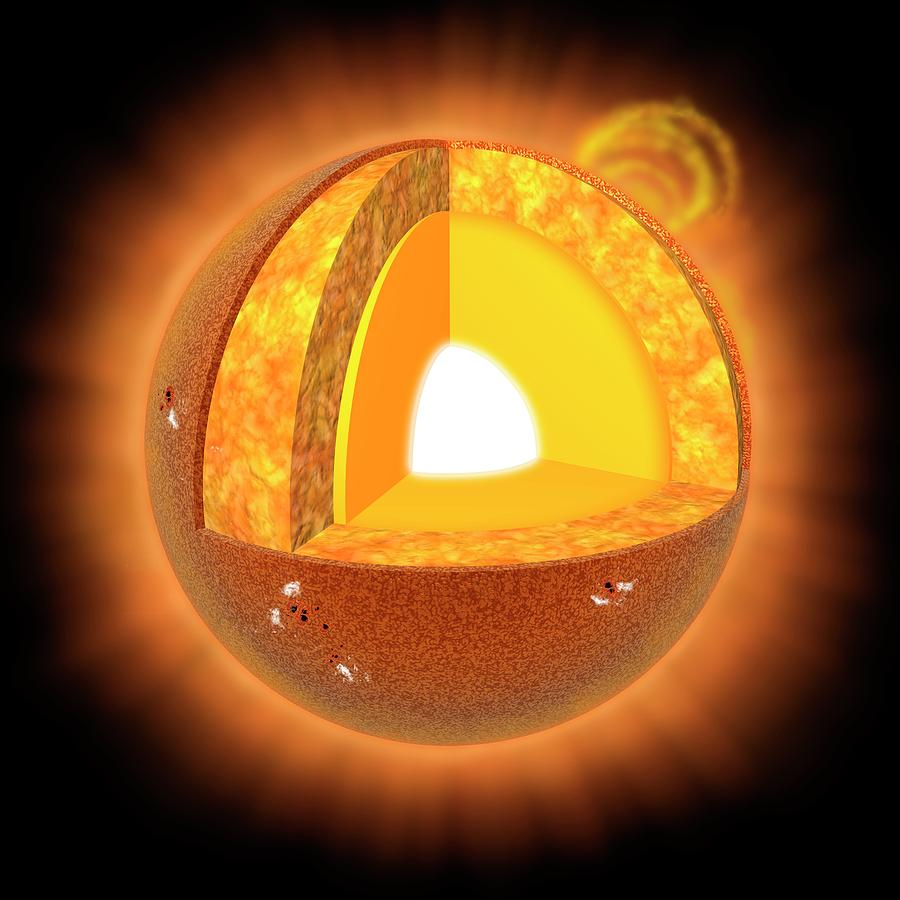
\includegraphics{img/sun_structure.jpg} \\
\captionsetup{labelformat=empty}
\caption{Звезда главной последовательности, $\varnothing \approx 0,01 \; \mathrm{\text{АЕ}}$}

\end{figure}
}
\only<2>{
\begin{figure}
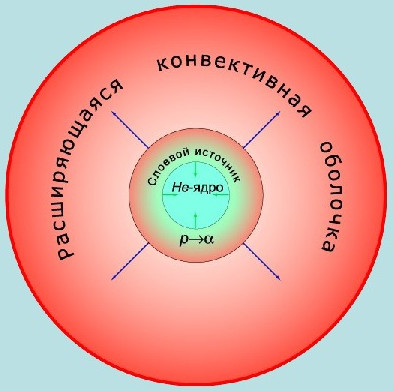
\includegraphics[width=\textwidth,height=\textheight,keepaspectratio]{img/red_giant_inert_helium.jpg} \\
\captionsetup{labelformat=empty}
\caption{Красный гигант}
\end{figure}
}
\only<3>{
\begin{figure}
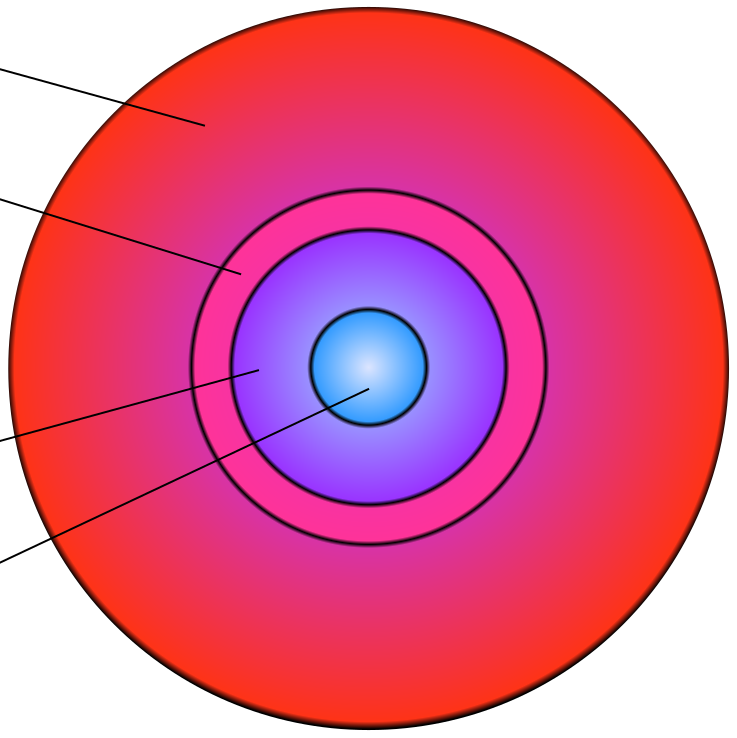
\includegraphics[width=\textwidth,height=\textheight,keepaspectratio]{img/red_giant_helium_burning.png} \\
\captionsetup{labelformat=empty}
\caption{Красный гигант, $\varnothing \approx 1 \; \mathrm{\text{АЕ}}$}
\end{figure}
}
\end{columns}
\end{frame}

\section{Прекрасное далёко}
\begin{frame}
\frametitle{Добейте выживших}
\begin{columns}[c]
\column{0.65\textwidth}
\begin{block}{$\Lambda-\mathrm{CDM}$}
Вечное ускоренное расширение
\end{block}
\begin{block}{600 млрд. лет}
Все галактики за космологическим горизонтом
\end{block}
\begin{block}{100 трлн. лет}
Погаснет последняя зведа
\end{block}
\begin{block}{$10^{15}$ лет}
Развал планетарных систем
\end{block}
\begin{block}{$10^{100}$ лет}
Испарится последняя чёрная дыра
\end{block}
\column{0.33\textwidth}
\only<2->{
\begin{block}{Тепловая смерть}
Ничего не происходит. \\
\only<3>{
\begin{center}
Вся Вселенная -- \\
\vspace{10pt}
{\usebeamercolor[fg]{title}\huge{СКУЧНОЕ}} \\
место
\end{center}
}
\end{block}
}
\vfill
\end{columns}
\end{frame}

\section{Литература}
\begin{frame}[allowframebreaks]
\footnotesize{

\begin{thebibliography}{99}
\bibitem{arXiv:astro-ph/0309415}%
A. Melott, B. Lieberman, C. Laird, L. Martin, M. Medvedev, B. Thomas (University of Kansas), J. Cannizzo, N. Gehrels, C. Jackman (NASA-Goddard) 
\newblock Did a gamma-ray burst initiate the late Ordovician mass extinction?
\newblock \href{http://arxiv.org/abs/astro-ph/0309415}{astro-ph/0309415}

\bibitem{arXiv:2302.13383}%
D. Frederiks, D. Svinkin, A. L. Lysenko, S. Molkov, A. Tsvetkova, M. Ulanov, A. Ridnaia, A. A. Lutovinov, I. Lapshov, A. Tkachenko, V. Levin
\newblock Properties of the extremely energetic GRB~221009A from Konus-\textit{WIND} and \textit{SRG}/ART-XC observations
\newblock \href{http://arxiv.org/abs/2302.13383}{arXiv:2302.13383}


\bibitem{arXiv:0911.4872}I. Ribas (2009)
\newblock The Sun and stars as the primary energy input in planetary atmospheres
\newblock \href{http://arxiv.org/abs/0911.4872}{arXiv:0911.4872}

\bibitem{arXiv:0912.2482}Martin J. Heath, Laurance R. Doyle
\newblock Circumstellar Habitable Zones to Ecodynamic Domains: A Preliminary Review and Suggested Future Directions
\newblock \href{http://arxiv.org/abs/0912.2482}{arXiv:0912.2482}

\bibitem{Bounama}Bounama, C., Franck, S., and von Bloh, W. (2001)
\newblock The fate of Earth's ocean
\newblock \href{http://doi.org/10.1016/0019-1035(88)90116-9}{Hydrol. Earth Syst. Sci., 5, 569-576}

\bibitem{James F. Kasting}
\newblock Runaway and moist greenhouse atmospheres and the evolution of Earth and Venus
\newblock \href{https://doi.org/10.1016/0019-1035(88)90116-9}{Icarus (ISSN 0019-1035), vol. 74, June 1988, p. 472-494.}

\bibitem{arXiv:1205.6864}Roeland P. van der Marel, Mark Fardal, Gurtina Besla, Rachael L. Beaton, Sangmo Tony Sohn, Jay Anderson, Tom Brown, Puragra Guhathakurta
\newblock The M31 Velocity Vector. II. Radial Orbit Towards the Milky Way and Implied Local Group Mass
\newblock \href{http://arxiv.org/abs/1205.6863}{arXiv:1205.6864}

\bibitem{arXiv:1805.04079}Roeland P. van der Marel, Mark A. Fardal, Sangmo Tony Sohn, Ekta Patel, Gurtina Besla, Andrés del Pino-Molina, Johannes Sahlmann, Laura L. Watkins
\newblock First Gaia Dynamics of the Andromeda System: DR2 Proper Motions, Orbits, and Rotation of M31 and M33
\newblock \href{http://arxiv.org/abs/1805.04079}{arXiv:1805.04079}

\bibitem{arXiv:astro-ph/0509839}Ralf Bender, John Kormendy, Gary Bower, Richard Green, Jens Thomas, Anthony C. Danks, Theodore Gull, J. B. Hutchings, C. L. Joseph, M. E. Kaiser, Tod R. Lauer, Charles H. Nelson, Douglas Richstone, Donna Weistrop, Bruce Woodgate
\newblock HST STIS spectroscopy of the triple nucleus of M31: two nested disks in Keplerian rotation around a Supermassive Black Hole
\newblock \href{http://arxiv.org/abs/astro-ph/0509839}{arXiv:astro-ph/0509839}

\end{thebibliography}
}
\end{frame}

\end{document} 
